\documentclass[a4paper,twoside,12pt,chapterprefix=false,bibliography=totocnumbered]{scrbook}
\usepackage{lmodern}
\usepackage{amssymb,amsmath}
\usepackage{ifxetex,ifluatex}
\usepackage{fixltx2e} % provides \textsubscript
\ifnum 0\ifxetex 1\fi\ifluatex 1\fi=0 % if pdftex
  \usepackage[T1]{fontenc}
  \usepackage[utf8]{inputenc}
\else % if luatex or xelatex
  \ifxetex
    \usepackage{mathspec}
  \else
    \usepackage{fontspec}
  \fi
  \defaultfontfeatures{Ligatures=TeX,Scale=MatchLowercase}
\fi
% use upquote if available, for straight quotes in verbatim environments
\IfFileExists{upquote.sty}{\usepackage{upquote}}{}
% use microtype if available
\IfFileExists{microtype.sty}{%
\usepackage[]{microtype}
\UseMicrotypeSet[protrusion]{basicmath} % disable protrusion for tt fonts
}{}
\PassOptionsToPackage{hyphens}{url} % url is loaded by hyperref
\usepackage[unicode=true]{hyperref}
\hypersetup{
            pdftitle={Second Language Acquisition: a corpus-based approach for a theoretical investigation},
            pdfauthor={Marco Petolicchio},
            pdfborder={0 0 0},
            breaklinks=true}
\urlstyle{same}  % don't use monospace font for urls
\usepackage{natbib}
\bibliographystyle{apa}
\usepackage{longtable,booktabs}
% Fix footnotes in tables (requires footnote package)
\IfFileExists{footnote.sty}{\usepackage{footnote}\makesavenoteenv{long table}}{}
\usepackage{graphicx,grffile}
\makeatletter
\def\maxwidth{\ifdim\Gin@nat@width>\linewidth\linewidth\else\Gin@nat@width\fi}
\def\maxheight{\ifdim\Gin@nat@height>\textheight\textheight\else\Gin@nat@height\fi}
\makeatother
% Scale images if necessary, so that they will not overflow the page
% margins by default, and it is still possible to overwrite the defaults
% using explicit options in \includegraphics[width, height, ...]{}
\setkeys{Gin}{width=\maxwidth,height=\maxheight,keepaspectratio}
\IfFileExists{parskip.sty}{%
\usepackage{parskip}
}{% else
\setlength{\parindent}{0pt}
\setlength{\parskip}{6pt plus 2pt minus 1pt}
}
\setlength{\emergencystretch}{3em}  % prevent overfull lines
\providecommand{\tightlist}{%
  \setlength{\itemsep}{0pt}\setlength{\parskip}{0pt}}
\setcounter{secnumdepth}{5}
% Redefines (sub)paragraphs to behave more like sections
\ifx\paragraph\undefined\else
\let\oldparagraph\paragraph
\renewcommand{\paragraph}[1]{\oldparagraph{#1}\mbox{}}
\fi
\ifx\subparagraph\undefined\else
\let\oldsubparagraph\subparagraph
\renewcommand{\subparagraph}[1]{\oldsubparagraph{#1}\mbox{}}
\fi

% set default figure placement to htbp
\makeatletter
\def\fps@figure{htbp}
\makeatother

\usepackage[a4paper,left=4cm, top=3cm, bottom=3cm, right=4cm, heightrounded, headsep=2em,
footskip=11mm, vmarginratio=1:1]{geometry}


\usepackage{fontspec}

\usepackage{ifluatex}

\usepackage{microtype}


\setmainfont[Numbers=Lowercase]{IBMPlexSerif-Light}
\setsansfont[Numbers=Lowercase]{IBMPlexSans-Light}
\setmonofont[Numbers=Lowercase]{IBMPlexMono-Light}


\usepackage[english]{babel}


\usepackage[usenames, dvipsnames]{color}
\definecolor{upol-dGrey}{rgb}{0.36470588235,0.36862745098,0.37647058823}
\definecolor{upol-lGrey}{rgb}{0.8,0.8,0.8}
\definecolor{upol-brandBlue}{rgb}{0,0.43529411764,0.67843137254}


\usepackage{xcolor}
\usepackage{graphicx}
\definecolor{titlepagecolor}{cmyk}{1,.38,0,.15} %C100 M38 Y0 K15
\definecolor{namecolor}{cmyk}{0, 0, 0, .0980} 
\usepackage{textcase}


\usepackage{setspace}

\makeatletter\let\Title\@title\makeatother
\makeatletter\let\Author\@author\makeatother



\usepackage{sectsty}
\allsectionsfont{\color{upol-dGrey}\sffamily}
\chapterfont{\color{upol-dGrey}\raggedleft\thispagestyle{empty}}







\makeatletter
\def\verbatim@font{\linespread{1}\footnotesize\ttfamily}
\makeatother



\makeatletter
\renewenvironment{figure}[1][\fps@figure]{
  \edef\@tempa{\noexpand\@float{figure}[#1]} 
  \@tempa
  \sffamily
}{
  \end@float
}
\renewenvironment{table}[1][\fps@table]{
  \edef\@tempa{\noexpand\@float{table}[#1]} 
  \@tempa
  \sffamily
  \footnotesize
}{
  \end@float
}
\makeatother

\usepackage{tabularx}
\usepackage{amsfonts}
\usepackage{booktabs}
\usepackage{siunitx}
\usepackage{fancyhdr}

\usepackage{lipsum, kantlipsum} % just for testing

\pagestyle{fancy}
\fancyhf{}
\fancyhead[LE,RO]{\thepage}
\fancyhead[RE]{\footnotesize\nouppercase{\leftmark}}
\fancyhead[LO]{\footnotesize\nouppercase{\rightmark}}
\setlength{\headheight}{14.5pt} % as requested by fan
\renewcommand{\headrulewidth}{0pt}

\renewcommand{\chaptermark}[1]{\markboth{\thechapter \ . \  #1}{}}
\renewcommand{\sectionmark}[1]{\markright{\thesection \ \ #1}{}}





%\setcounter{secnumdepth}{5}
%\setsecnumdepth{subsubsection}
%\maxtocdepth{subsubsection}


\setlength{\skip\footins}{3em}
\renewcommand\footnoterule{{\hrule height 0pt}} % a long blue line



\usepackage{colortbl}
\arrayrulecolor{gray}









\usepackage{pdfpages}






%Options: Sonny, Lenny, Glenn, Conny, Rejne, Bjarne, Bjornstrup
\usepackage[Bjornstrup]{fncychap}
%\renewcommand{\CNoV}{\raggedleft\sffamily\selectfont\HUGE}
  \ChNumVar{\Huge\sffamily\selectfont}
\renewcommand{\DOCH}{%
   \settowidth{\py}{\CNoV\thechapter}
  \addtolength{\py}{1em}      % Amount of space by which the
%                                % number is shifted right
   \fboxsep=0pt%
   \colorbox[gray]{.85}{\rule{0pt}{50pt}\parbox[b]{\textwidth}{\hfill}}%
   \kern-\py\raise20pt%
   \hbox{\color{gray}\CNoV\thechapter}\\%
}

\makeatletter
\renewcommand*{\@makechapterhead}[1]{%
  \vspace*{0\p@}%
  {\parindent \z@ \raggedright \normalfont
    \ifnum \c@secnumdepth >\m@ne
      \if@mainmatter%%%%% Fix for frontmatter, mainmatter, and backmatter 040920
        \DOCH
      \fi
    \fi
    \interlinepenalty\@M
    \if@mainmatter%%%%% Fix for frontmatter, mainmatter, and backmatter 060424
      \DOTI{#1}%
    \else%
      \DOTIS{#1}%
    \fi
  }}
% For the case \chapter*:
\renewcommand*{\@makeschapterhead}[1]{%
  \vspace*{10\p@}%
  {\parindent \z@ \raggedright
    \normalfont
    \interlinepenalty\@M
    \DOTIS{#1}
    \vskip 0\p@
  }}
\makeatother




\renewcommand*\chapterpagestyle{empty}




\usepackage{tikz,tikz-qtree}

\usepackage{listings}
\lstset{ %Formatting for code in appendix
	backgroundcolor = \color{gray},
	language=Python,
	basicstyle=\singlespacing\footnotesize\ttfamily\color{white},
	numbers=left,
	stepnumber=1,
	showstringspaces=true,
	tabsize=2,
	breaklines=true,
	breakatwhitespace=false,
	xleftmargin=3em,framexleftmargin=3em, numberstyle=\ttfamily,
}

\usepackage{datetime}

\let\oldmaketitle\maketitle
\AtBeginDocument{\let\maketitle\relax}

\usepackage[autostyle]{csquotes}  
\usepackage{enumerate}



\usepackage{tikz}
\usepackage{pgfplots}


\usepackage{gb4e,cgloss}
\noautomath

\frontmatter

\title{Second Language Acquisition: a corpus-based approach for a theoretical
investigation}
\author{Marco Petolicchio}
\date{2018-05-29}

\usepackage{amsthm}
\newtheorem{theorem}{Theorem}[chapter]
\newtheorem{lemma}{Lemma}[chapter]
\theoremstyle{definition}
\newtheorem{definition}{Definition}[chapter]
\newtheorem{corollary}{Corollary}[chapter]
\newtheorem{proposition}{Proposition}[chapter]
\theoremstyle{definition}
\newtheorem{example}{Example}[chapter]
\theoremstyle{definition}
\newtheorem{exercise}{Exercise}[chapter]
\theoremstyle{remark}
\newtheorem*{remark}{Remark}
\newtheorem*{solution}{Solution}
\begin{document}
\maketitle

\begin{titlepage}
\pagecolor{titlepagecolor}
\noindent
\color{white}
\makebox[0pt][l]{\rule{1.4\textwidth}{1pt}}
\par
\noindent
\textbf{\sffamily{Palacký University}} \textcolor{namecolor}{\sffamily{ Olomouc}}\par \vskip\baselineskip 
\noindent\sffamily{Ph.D. Thesis in Italian Linguistics} \\
\noindent\sffamily{Dept. of Romance Languages, Faculty of Arts} \par

\vfill

\noindent
{\Huge \sffamily{Second Language Acquisition: \\ 
a corpus based approach \\ 
for a theoretical investigation

}} \par
\vskip\baselineskip
\noindent
\MakeTextUppercase{\large\sffamily{Marco Petolicchio}} \par \vskip\baselineskip
\noindent
\vfill
\noindent
{\Large \sffamily{Supervisors}}\par \vskip\baselineskip
\noindent
\sffamily{\MakeTextUppercase{Dr. Lorem Ipsum} \\ Palacký University \\ \textcolor{namecolor}{Dept. of Romance Languages, Faculty of Arts} }\par \vskip\baselineskip
\noindent
\sffamily{\MakeTextUppercase{Prof. Dolorem Sit Amet} \\ University of Lorem\\ \textcolor{namecolor}{Dept. of Lorem Ipsum, Faculty of Humanities} }\par \vskip\baselineskip
\vfill
 {\footnotesize   \ttfamily{draft : : \today   : :  \currenttime} \par}

\end{titlepage}
\nopagecolor% Use this to restore the color pages to white
\pagecolor{white}

{
\setcounter{tocdepth}{1}
\tableofcontents
}
\listoftables
\listoffigures
\chapter*{Preface}\label{preface}
\addcontentsline{toc}{chapter}{Preface}

\section*{Abstract}\label{abstract}
\addcontentsline{toc}{section}{Abstract}

The main topic of this doctoral dissertation is on the analysis of
syntactic structures in language acquisition, specifically in the domain
of Czech and Slovak learners which acquire the Italian language. In
particular, I will focus on the complex noun phrase subdomain, showing
the compositionality of the phrase structure and the hierarchical
fashion of this component. The analysis is casted in the
Minimalist-oriented framework of the Generative Grammar
\citep{chomsky1995, chomsky1998, chomsky2013, hcf2002} and its
application in the field of the second language acquisition
\citep{rothmanSlabakova2017, slabakovaLealLiskin2014}.

The usage of an established computational ground to conduct the work,
where the data retrieved by fieldwork is stored in a coherent corpus
which easily permits to be queried and interpolated for the research
purposes, represents a standpoint for this research in its totality,
yielding for a data-based approach to the whole process. The annotation
schema of the data is standardized in order to adhere to the major point
of discussion into the discipline
\citep{clark2010, kueblerZinsmeinster2015, kurdi2016}, representing the
plus to furnish a data source which is independent to the merely
contingent purposes.

This research aims to offer a way to investigate how second language
acquisition can be seen grounding on a coherent set of data in terms of
annotation schema: it does insist either on the speculative questions
both on computational models involved.

\section*{Keywords}\label{keywords}
\addcontentsline{toc}{section}{Keywords}

\begin{itemize}
\tightlist
\item
  Computational Linguistics
\item
  Syntax
\item
  Second Language Acquisition
\item
  Italian L2
\item
  Corpus Linguistics
\end{itemize}

\mainmatter

\chapter{Introduction}\label{introduction}

The main question of this thesis yields a twofold mindset that is not a
corollary of the research but which represents the process in which the
work was conducted: how could I investigate a particular area of the
language faculty as language acquisition in a way which can gain from
the usage of the digital instruments in order to ground the theoretical
analysis on actual data?

The idea under this research moves across the motivation to investigate
over an empirically-grounded path the strategies shown by the learners
during the acquisition of second languages, using an established
coherent digital architecture. My task is twofold: on one side this
provides for the developing of a theoretically-grounded framework to
research in the fields of Second Language Acquisition (SLA), while on
the other this necessitates to develop a linguistic corpus which collect
in a coherent fashion a wide set of data that represent some spotted
linguistic facts in order to give a transparent documentation of the
learning path. The usage of the modern tools in developing a linguistic
corpus yields for a fully documentable research path, in which is
possible to reconstruct the steps and the choices which underlie its
development, the methods used in the analysis, the correctness of the
outcomes. This kind of research is intimately multidisciplinar in
nature, embracing different approaches and areas of interest: digital
humanities, corpus and computational linguistics for the development of
the linguistic corpus, general and theoretical linguistics, studies on
SLA and interlanguage for the theoretical analysis.

This introductive chapter collects a preliminary way to represent the
main areas of the research, the methods involved in the analysis and the
possible outcomes of such a way to conduct the work.

\section{Background for the thesis}\label{background-for-the-thesis}

\subsection{Data-based research:
definition}\label{data-based-research-definition}

\subsection{Data-based research: motivations for the
thesis}\label{data-based-research-motivations-for-the-thesis}

\section{Objectives of the thesis}\label{objectives-of-the-thesis}

The three main objectives of this thesis are methodological, empirical
and theoretical.

\begin{enumerate}
\def\labelenumi{\arabic{enumi}.}
\tightlist
\item
  \textbf{Methodological objectives}\\
  To address the decision and the methods raised by the compilation, the
  storage and the design of a learner based corpus, exploring the
  effective procedures for retrieving the relevant features for the
  analysis;
\item
  \textbf{Empirical objectives}\\
  To explore the previous generalizations of the acquisitional path in
  SLA literature comparing with the amount of linguistic productions
  given by different learners;
\item
  \textbf{Theoretical objectives}\\
  To describe the features which are relevant for characterise the
  language variety effect and the place of interlanguage.
\end{enumerate}

\subsection{Methodological objectives}\label{methodological-objectives}

\subsection{Empirical objectives}\label{empirical-objectives}

Amongst many scholar the role of the native language (L1) has been
raised as a factor of possible conditionation in the way which the
target language (L2) is acquired during the learning path: an emblematic
case is the \emph{transfer} of the knowledge about the structures of the
L1 to the target, revealing the intermediate steps of the acquisitional
path defined with the term \emph{interlanguage} \citep{selinker1972},
that we can refer as to \textbf{Interlanguage Hypothesis} (IlH).
Different from this hypothesis --which recognizes a central place to the
native language in the acquisitional path-- is the \textbf{Monitor
Model} \citep{krashen1981}, a multi-focal perspective on language
acquisition where different factors are described as involved in the
process and where the L1 could not represent that conditionation.

During the last 20 years, a considerable part of linguistic literature
is involved in developing some sort of models to think how the faculty
of language can work, in its biological \citep{hcf2002}, computational
\citep{fodor2001} and cognitive components in a highly interdisciplinary
environment. Studies on SLA is a fertile field, which relies on
comparative and contrastive analyses of linguistic phenomena, either
both from an applied view \citep{ellis1994} than by theoretically
grounded perspective focused on Generative framework (GenSLA)
\citep{guasti2002, hawkins2001, rothmanSlabakova2017, sorace2011}. In
this sense appears that the adoption of a coherent framework to analyze
the variation in grammar into a \emph{parametric} model
\citep{chomsky1995} can be suitable for long-standing researches on SLA
and interlanguage, also based on independent data-mining initiatives as
in the case of the present purposes, which disentangles the data in a
form of a linguistic corpus and the linguistic analysis.

The dataset used in this thesis aims to display either the different
linguistic outcomes in a wide range of communicative situations by the
same learner, both than a sociolinguistic grained analysis where the
variety of educational or age range can show different linguistic
behaviors.

\subsection{Theoretical objectives}\label{theoretical-objectives}

From a theoretical viewpoint, the research is inserted in the current
theories that rely on the hierarchical functioning of the language
faculty, for which the variation among languages are reconducted to a
parametrizing of choice among the structures of languages
\citep{adger2013, chomsky1995, chomsky1998, chomsky2013, chomsky2015, rizzi2013},
which are constant between the language structures, despite of the
wideness of the variation amongst the languages:

\begin{quote}
We are concerned, then, with states of the language faculty, which we
understand to be some array of cognitive traits and capacities, a
particular component of the human mind/brain. The language faculty has
an initial state, genetically determined; in the normal course of
development it passes through a series of states in early childhood,
reaching a relatively stable steady state that undergoes little
subsequent change, apart from the lexicon. To a good first
approximation, the initial state appears to be uniform for the species.
\citep{chomsky1995}
\end{quote}

This view permits on one side to compare the syntactic structures in a
coherent and schematic way, while on the other it concentrates moreover
on the hierarchical fashion of the language faculty than on the linear
order displayed by the utterances \citep{kayne1994, moro2000}. In this
perspective is generally assumed that the hierarchical phrase structure
plays a central role in syntactic computation, while the
\emph{flattering} of such structures into a mono-dimensional workspace
is a matter of externalization constraints and interface conditions
(e.g.~the need to give an ordered array where every item of the sentence
is present at one time in order to be spelled out). I will summarize
this in a representational way with the usual tree-diagram in
Fig.\ref{fig:tree1}.

\begin{figure}
\centering
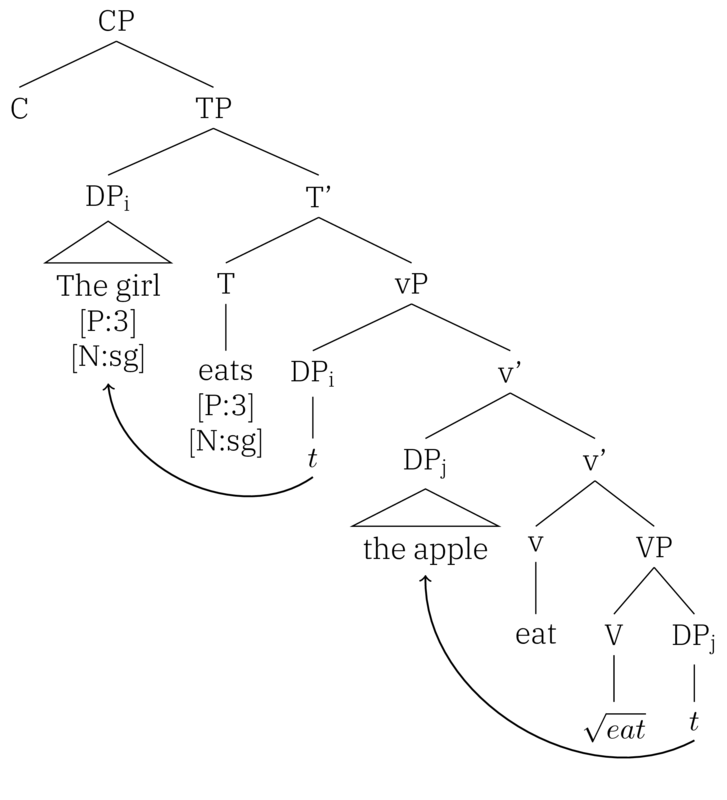
\includegraphics{./assets/img/png-tree1.png}
\caption{\label{fig:tree1} Representation of syntactic structures}
\end{figure}

Given this way to proceed, that assure a coherent framework to compare
languages in a parametric way, the main theoretical question addressed
here concerns the relevance and the potential usage of this perspective
in the analysis of a dynamic system as during the acquisitional path and
the strategies raised up by learners during the various steps in the
interlanguage.

\section{Outline of the thesis}\label{outline-of-the-thesis}

The first year is dedicated to the setting-up of the corpus, with the
starting operations to acquire the data and elaborate a coherent way to
annotate the texts with a standard schema. During the second year the
corpus is planned to grow up for reach a significance level of
\textgreater{}15000 words in order to provide quantitative analyses.
Third and fourth year will be spent in developing the theoretical
analyses and refining the informatic architecture of the project,
evolving in a user-friendly and interrogable way to dispense the data.
The theoretical outcome constitues the main topic of the research.

\textbf{Chapter 2} introduces \ldots{}

\textbf{Chapter 3} introduces \ldots{}

\textbf{Chapter 4} introduces \ldots{}

\textbf{Chapter 5} introduces \ldots{}

\backmatter

\chapter*{Backmatter}\label{backmatter}
\addcontentsline{toc}{chapter}{Backmatter}

\section*{Credits}\label{credits}
\addcontentsline{toc}{section}{Credits}

This project is constituted by files written in Markdown syntax and
exported either as a standalone website both as printer-ready product.
This is due to the awesome work of the people behind different
libraries:

\begin{itemize}
\tightlist
\item
  \href{https://bookdown.org}{Pandoc}
\item
  \href{https://bookdown.org}{Bookdown}
\item
  \href{https://bookdown.org}{RMarkdown} and
  \href{https://bookdown.org}{R} environment.
\end{itemize}

As well, for the computational infrastructure, a lot of open source
tools have been used:

\begin{itemize}
\tightlist
\item
  \href{https://bookdown.org}{NLTK}
\end{itemize}

For the typographic setting, the print-ready file is composed on LaTeX
with the usage of SCRBOOK class and some custom component. I am aware I
can't thank everyone on the web about that. By the way, thank you!

\section*{About the author}\label{about-the-author}
\addcontentsline{toc}{section}{About the author}

I am a Graduate Researcher involved in a Ph.D.~Program in Italian
Linguistics at the Department of Romance Studies in the Faculty of
Phylosophy at Palacky University in Olomouc, Czech Republic.

My interests span across digital humanities, syntax theories and
computational linguistics.

Feel free to write me at
\href{mailto:marco.petolicchio@gmail.com}{\nolinkurl{marco.petolicchio@gmail.com}}
or visit marcopetolicchio.com for the detailed contact list.

\bibliography{bibliography.bib}

\end{document}
